\chapter[Introduction]{Introduction}
\def\chpname{intro}\label{chp:\chpname}

Chapter editors:
\credit{bethwillman},
\credit{connolly},
\credit{ivezic},
\credit{drphilmarshall}.

The Large Synoptic Survey Telescope (LSST) is a dedicated optical
telescope with an effective aperture of 6.7 meters, currently under
construction on Cerro Pach\'on in the Chilean Andes.  The telescope
and camera will have a huge field of view, 9.6 deg$^2$, and the
\'etendue, i.e., the product of collecting area and field of view will
be significantly larger than any other optical telescope.  Thus this telescope
is designed for wide-field deep imaging of the sky; its mantra is
``Wide-Deep-Fast'', i.e., the ability to cover large swaths of sky
(``Wide'') to faint magnitudes (``Deep'') in a short amount of time
(``Fast''), allowing it to scan the sky repeatedly.  LSST will image
in six broad filters, $ugrizy$, spanning the optical band from the
atmospheric cutoff in the ultraviolet to the limit of CCD sensitivity
in the near-infrared.

The science case for the LSST is based broadly on four science themes:
\begin{itemize}
\item Dark energy and dark matter (via measurements of strong and weak lensing,
  large-scale structure, clusters of galaxies, and supernovae);
\item Exploring the transient and variable universe;
\item Studying the structure of the Milky Way galaxy and its neighbors
  via resolved stellar populations;
\item An inventory of the Solar System, including Near Earth Asteroids
  and Potential Hazardous Objects, Main Belt Asteroids, and
  Kuiper Belt Objects.
\end{itemize}

These themes, together with {\em many} other science applications, are
described in detail in the
\href{http://lsst.org/scientists/scibook}{LSST Science Book}, produced
by the LSST Project Team and Science collaborations in 2009.  The
present white paper represents an important next step in science
planning beyond the Science Book.  In particular, we now need to
quantify how well the LSST (for a given realization of its observing
strategy, or ``{\em cadence}'') will be able to carry out its science
goals; indeed, we will use this quantification to refine and optimize
the cadence itself.  To zeroth order, the large \'etendue of LSST
allows it to meet all its science goals with a single dataset with a
universal cadence.  This document describes the design of the LSST
cadence and the various ways in which can be further refined to
optimize the science output of the survey.  As we describe in detail
below, we quantify the effectiveness of a given cadence realization to
meet science goals by defining a series of quantitative {\em metrics}.
Any given realization will be more favorable for some science areas,
and less so for others; the metrics allow us to quantify this, and
optimize the overall cadence for the broadest range of LSST science
areas.

In the six years since the Science Book was written, some of the
science themes described in there have evolved or become obsolete,
while new science opportunities and ideas have arisen.  Moreover, our
understanding of the capabilities (such as system response and
therefore depth, telescope optics, and so on) have matured
considerably.  The present document endeavors to explore the principal
science themes as described in the Science Book, but is not slaved to
them, and where appropriate, we will point out relevant updates to the
Science Book.



% --------------------------------------------------------------------

\section{Synoptic Sky Surveying at Universal Cadence}
\def\secname{intro:baseline}\label{sec:\secname}

\credit{ivezic},
\credit{drphilmarshall},
\credit{michaelstrauss}


The LSST defined a so-called ``baseline cadence'', described in the
\href{http://adsabs.harvard.edu/abs/2008arXiv0805.2366I}{LSST overview
paper} and Chapter 3 of the Science Book.  This was used
to demonstrate that LSST could meet its basic science goals, and indeed
the formal
\href{https://www.lsstcorp.org/docushare/dsweb/Get/LPM-17}{science
requirements}.    As described in these references, the default LSST
exposure is 15 seconds, and all exposures are taken in pairs, called a
``{\em visit}'', before the telescope is slewed to a neighboring field.
Any given field is observed twice on a given night, which allows
preliminary trajectories of asteroids to be determined.

The baseline cadence optimizes the amount of sky covered in any given
night (subject to the constraint of observing at airmass less than 1.4
throughout), and allows the entire sky visible at any time of the year
to be covered in about three nights.  The cadence is designed to give
uniform coverage at any given time, and reaches survey goals for
measuring stellar parallax and proper motion over the ten-year survey.
The survey requirements on depth lead to roughly 825 visits (summing
over the six filters) in the 10-year LSST survey to any given point on
the sky.  The resulting Deep-Wide-Fast component of the survey covers
roughly 18,000 deg$^2$ of high Galactic latitude sky, and requires about
85\% of the available observing time.

There are obvious science cases that the Deep-Wide-Fast survey does
not address, and thus the remaining 15\% of the telescope time in the
baseline cadence is devoted to a series of specialized surveys.  They
are as follows:
\begin{itemize}
\item Imaging at low Galactic latitudes.  This is currently defined as
  a wedge which is broader closer to the Galactic Center,
  corresponding roughly to a locus of constant stellar density.  In
  this region, the number of repeat observations is reduced, given the
  confusion limit in the stacked LSST data.
\item Imaging in the South Celestial Cap.  The airmass limit of 1.4
  restricts observations to declination $> -75^\circ$, thus missing
  large fraction of both the Magellanic Clouds.
  Observations are done in the Cap to cover this region of sky, again
  to shallower depth.
\item Imaging in a series of four {\em Deep Drilling Fields}, single
  pointings in which
  we will obtain roughly 5 times more exposures in all
  filters in order to go about a magnitude fainter in the stacked
  data, as well as to get better sampled light curves of variable
  objects.
\item Imaging in the Northern portions of the Ecliptic Plane.  The
  airmass limit of 1.4 restricts us to declination $< +15^\circ$, which
  means that significant fraction of the Ecliptic Plane
  is uncovered.  By observing with a reduced cadence close to the
  Ecliptic Plane north of this limit, we will be able to significantly
  increase the fraction of Near-Earth Asteroids and Main Belt
  Asteroids for which LSST obtains orbits.
\end{itemize}

The LSST Project has developed an ``Operations Simulator'' (\OpSim),
% described in detail in Chapter~\ref{chp:cadexp} of this paper,
which
includes a realistic model of telescope operations, including time
required for camera readout, slew time, filter exchange, as well as time
loss due to clouds.  Given a set of so-called ``proposals''
that set the priorities of which fields to
observe at any given time, \OpSim has developed a series of realizations
of the series of observations that make up the ten-year LSST survey.
The baseline cadence is a specific realization of the
\OpSim output, which meets the LSST survey requirements, following the
rules briefly outlined above.

Again, while the baseline cadence demonstrates that the LSST is capable
of meeting its stated science goals, it is not optimized for all
science, and \autoref{chp:cadexp} of this document describes a
series of experiments varying the assumptions in \OpSim.  In
\autoref{chp:specialsurveys}, we explore additional ideas for future
experiments to be done in \OpSim -- many of them, we hope, inspired by
requests from the community.

\navigationbar

% --------------------------------------------------------------------

\section{Evaluating and Optimizing the LSST Observing Strategy}
\def\secname{intro:evaluation}\label{sec:\secname}

\credit{drphilmarshall}

Given a realization of the LSST observing strategy (i.e., an output of
\OpSim), our first task is to quantify how well it supports the (many)
science projects that LSST will enable.  As the algorithms controlling
\OpSim are varied, some projects will benefit, while others may suffer.
By quantifying this for each projects, we can determine which cadence
maximizes the science potential overall of the project.

Therefore, we need a {\it science-based evaluation of the baseline LSST
observing strategy and its variants}. After simulating a sample
observing schedule consistent with this strategy (see
\autoref{chp:cadexp}), we then need to quantify its value to each
science team.  This is what the LSST Simulations team's ``Metric
Analysis Framework'' was designed to enable: science case investigators
can now design quantitative evaluations of the outputs of \OpSim, to
answer the question, ``how good would that observing strategy be, for my
science?'' These ``metrics'' can be coded against the \MAF API, and
shared among the LSST science community at the
\href{https://sims-maf.lsst.io/metricList.html#contributed-mafcontrib-metrics}{\simsMafContrib}
online repository. All of the \MAF metrics described in this paper can
be found there.

Once the fiducial strategy has
been evaluated in this way, then any other strategy can be evaluated
in the same terms, using the same code.  We will then be able to iterate towards an
science-optimized strategy.

With this program in mind, it makes sense to define {\it one ``Figure
of Merit'' (FoM) per science project}, that captures the value of  the
observing strategy under consideration to that science team. This FoM
will probably be a function of several ``diagnostic metrics'' that quantify
lower-level features of the observing sequence.  For Figures of Merit
to be directly comparable between disparate science projects,  they
need to be dimensional, and have the same units.
\footnote{One natural choice of units for Figures of Merit could be the
{\it information  gained} by the science team, in bits. This is a
well-defined statistical quantity, albeit not yet one in common use.}
% A given observing schedule's value would then depend on both this
% information gain, but also {\it how much that information is worth to
% the whole community}. It is at this point that the debate could become
% heated: probably the best we could do in cadence diplomacy would be to
% to quantify all the information gains implied by each proposed change to
% the baseline  observing strategy, combine them to see whether it makes
% everyone happy, and iterate. In this way we might hope to minimize the
% debates about the less quantifiable worth of each piece of information.}

It may not always be straightforward to define a Figure of
Merit for some science cases, but the diagnostic metrics that they will likely depend
upon will be easier to derive. Writing this white paper is an
opportunity to think through the FoM for each science
project that we as a community want to carry out, and how that measure
of success is likely (or even known) to depend on metrics that
summarize the observing sequence presented to us. We return to the
question of FoM design in \autoref{sec:guidelines:metrics} below.

Thinking about the problem in terms of science projects, each with a
Figure of Merit, encourages us to design modular document sections, with
one science project and one Figure of Merit per section. These modular
sections ought then be easily extracted, combined and edited into
publishable articles. They will also naturally lead to the definition of
a suite of \MAF metrics that can be evaluated on any future \OpSim output
database.  Tabulating the values of the diagnostic metrics and the FoM,
for different cadences, for each science case, will be very helpful for
this purpose.

% --------------------------------------------------------------------

\section{Influencing the LSST Observing Schedule}
\label{sec:\secname:schedule}

What we find regarding the impact of various observing strategies on
science performance will be of great interest to the LSST project, as it
works towards defining the observatory's observing schedule. How will
the findings presented in this paper be taken forward?

In this section we describe the mechanisms by which community input to
the developing observing schedule will be absorbed, and explain how
we will distil the vital information that the project needs from our
\OpSim / \MAF analyses. We then provide a target timeline for the provision of community input.

% - - - - - - - - - - - - - - - - - - - - - - - - - - - - - - - - - - -

\subsection{How will the results of our analyses be used?}
\label{sec:\secname:useage}

\credit{bethwillman}, \credit{connolly}, \credit{ivezic}

Through the end of construction and commissioning, this community
Observing Strategy White Paper will remain a living document that is
{\it the vehicle for the community to communicate to the LSST Project
regarding the Wide-Fast-Deep and mini-survey observing strategies.}
{\it The Project Scientist will synthesize and act on the results
presented in this paper,} with support from the Science Advisory
Committee and Survey Strategy Committee (see below).

As described in the LSST Operations Plan (LPM-181), the observing
strategy will continue to be refined and optimized during operations:
the Survey Scientist will chair a survey evaluation working group that
will evaluate quarterly the current and expected performance of the
survey and scheduler software. This group may include representation
from the Survey Support Scientist, the Pipelines and Data Products
group, the Data Processing group, the Camera team, and science
community.  The science community representation may be implemented as a
sub-group of the Science Advisory Committee.

% - - - - - - - - - - - - - - - - - - - - - - - - - - - - - - - - - - -

\subsection{Communicating via Science Case Conclusions}
\label{sec:\secname:caseConclusions}

\credit{ivezic}

In order to consolidate the various constraints on the observing
strategy by different science cases, and provide high signal to noise
data for the project to take forward, each science case will answer ten
questions probing different aspects of the observing strategy, as
follows:

% AUTHORS! COPY AND PASTE THE FOLLOWING INTO YOUR SCIENCE SECTION!
%
% \subsection{Conclusions}
%
% Here we answer the ten questions posed in
% \autoref{sec:intro:evaluation:caseConclusions}:
%
\begin{description}

\item[Q1:] {\it Does the science case place any constraints on the
tradeoff between the sky coverage and coadded depth? For example, should
the sky coverage be maximized (to $\sim$30,000 deg$^2$, as e.g., in
Pan-STARRS) or the number of detected galaxies (the current baseline but
with 18,000 deg$^2$)?}

\item[A1:] ...

\item[Q2:] {\it Does the science case place any constraints on the
tradeoff between uniformity of sampling and frequency of  sampling? For
example, a rolling cadence can provide enhanced sample rates over a part
of the survey or the entire survey for a designated time at the cost of
reduced sample rate the rest of the time (while maintaining the nominal
total visit counts).}

\item[A2:] ...

\item[Q3:] {\it Does the science case place any constraints on the
tradeoff between the single-visit depth and the number of visits
(especially in the $u$-band where longer exposures would minimize the
impact of the readout noise)?}

\item[A3:] ...

\item[Q4:] {\it Does the science case place any constraints on the
Galactic plane coverage (spatial coverage, temporal sampling, visits per
band)?}

\item[A4:] ...

\item[Q5:] {\it Does the science case place any constraints on the
fraction of observing time allocated to each band?}

\item[A5:] ...

\item[Q6:] {\it Does the science case place any constraints on the
cadence for deep drilling fields?}

\item[A6:] ...

\item[Q7:] {\it Assuming two visits per night, would the science case
benefit if they are obtained in the same band or not?}

\item[A7:] ...

\item[Q8:] {\it Will the case science benefit from a special cadence
prescription during commissioning or early in the survey, such as:
acquiring a full 10-year count of visits for a small area (either in all
the bands or in a  selected set); a greatly enhanced cadence for a small
area?}

\item[A8:] ...

\item[Q9:] {\it Does the science case place any constraints on the
sampling of observing conditions (e.g., seeing, dark sky, airmass),
possibly as a function of band, etc.?}

\item[A9:] ...

\item[Q10:] {\it Does the case have science drivers that would require
real-time exposure time optimization to obtain nearly constant
single-visit limiting depth?}

\item[A10:] ...

\end{description}

\navigationbar


% - - - - - - - - - - - - - - - - - - - - - - - - - - - - - - - - - - -

\subsection{Timeline}
\label{sec:\secname:timeline}

\credit{connolly},
\credit{drphilmarshall}

%%%%%%%%%%%%%%%%%%%%%%%%%%%%%%%%%
\begin{figure}[ht!]
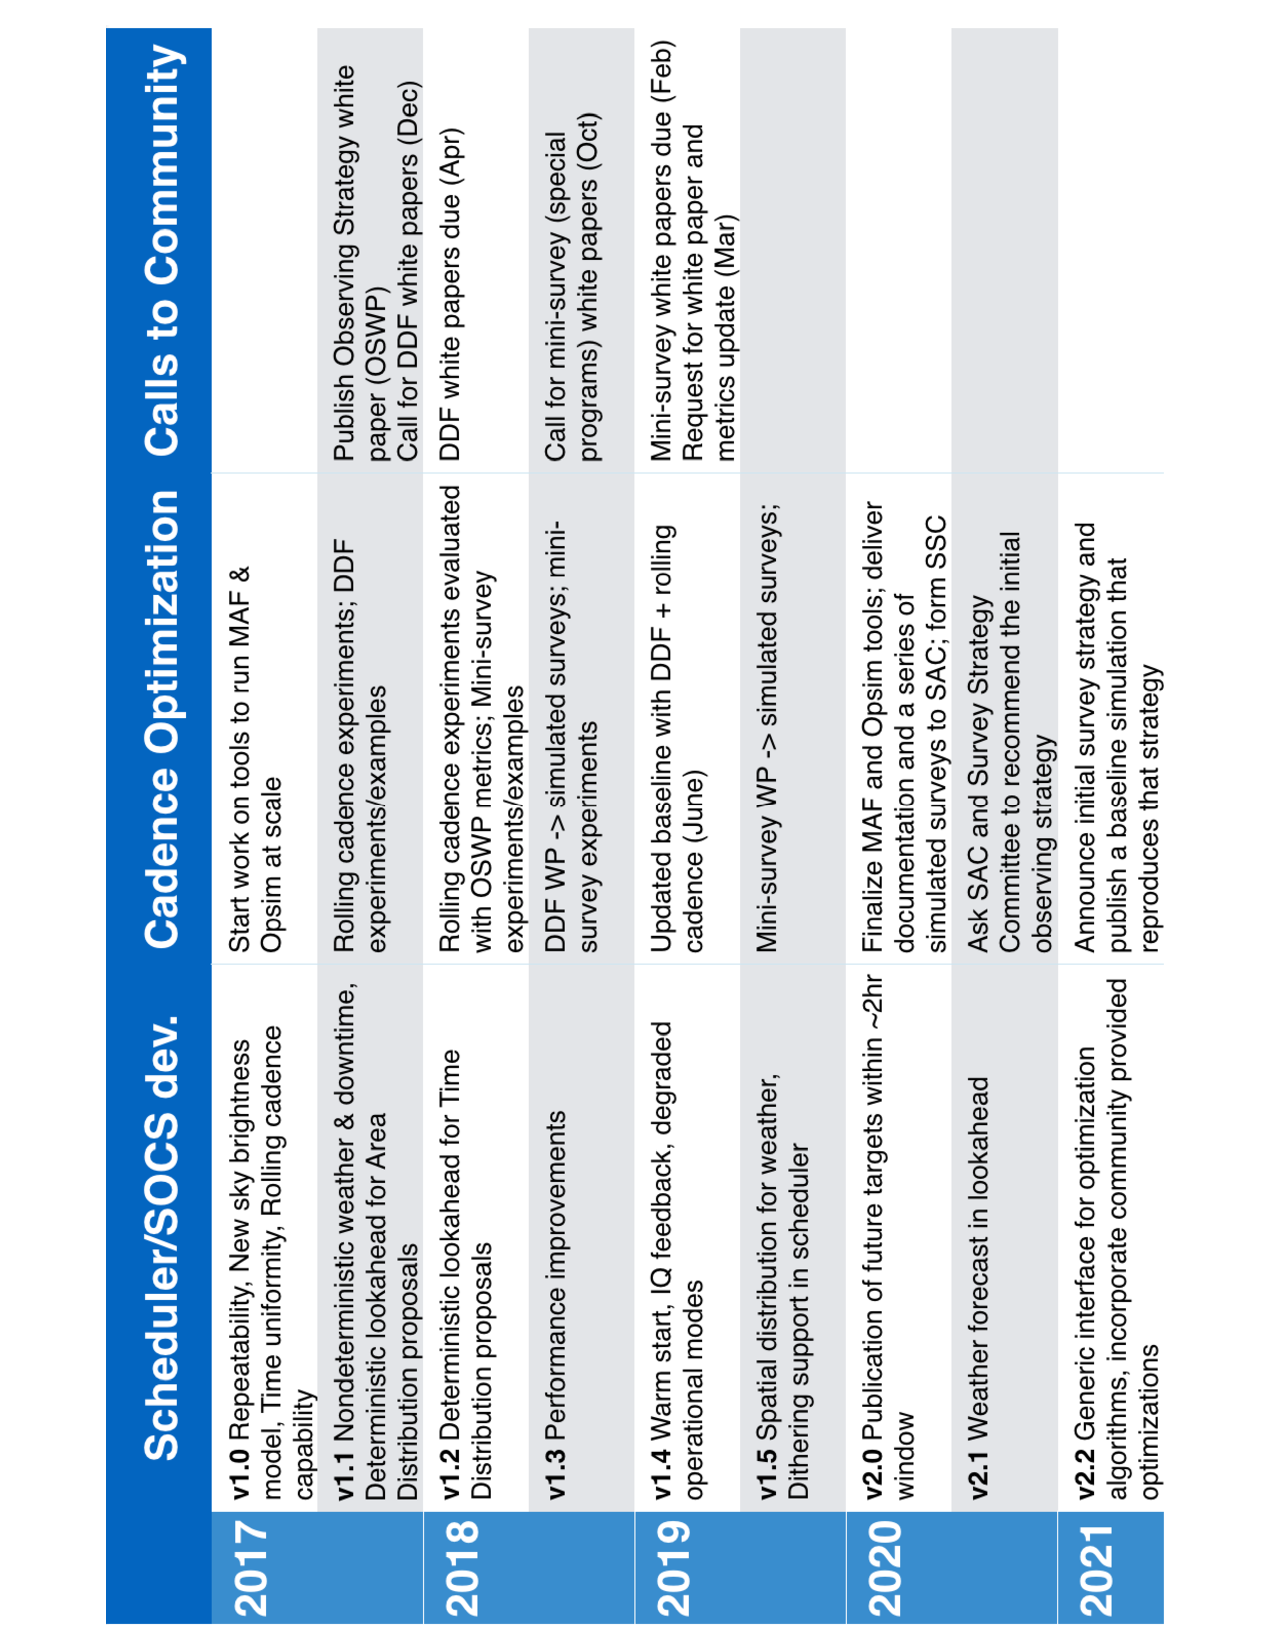
\includegraphics[angle=0,width=0.9\linewidth,clip]{figs/opsim_timeline.pdf}
\caption{Target timeline for the iterated optimization of the LSST observing strategy through 2020.}
\label{fig:timeline}
\end{figure}
%%%%%%%%%%%%%%%%%%%%%%%%%%%%%%%%%

The intersection between the community and the scheduler development,
and the expected support that can be provided by the Project, is
outlined in \autoref{fig:timeline}. From the point of view of the community, this timeline contains a number of interesting features:

\begin{description}

\item{\textbf{Update of the Baseline Cadence and Exploration of Rolling
Cadences.}} During development of version 1.0 of this white paper, the
Project has been developing an enhanced operations simulator code,
\OpSim~4. This will be used to generate, by September 2017, a new set of
observing strategies, including some that have a ``rolling cadence''
component. This is in response to the results presented in the science
chapters of this paper. Analysis of these simulations would form the
backbone of an updated, version 2.0 of this white paper, with existing
science cases being updated to include quantitative assessment of the
new \OpSim~4 simulations, and new science cases being identified and
investigated.

\item{\textbf{The definition of the Deep Drilling Fields (DDFs) and
associated cadences.}} The September 2017 simulations will all continue
to use the baseline DDF cadence. However, by September 2017, the LSST
will issue a call for proposals to define the cadence and properties of
the currently selected DDFs, and to propose a new set of DDFs. To enable
this, the project will publish the known boundary conditions for
additional DDFs (e.g.\ the definition of a DDF, the current division of
survey time, constraints on the number of filter exchanges that can be
accomplished within a night, the expected range of integration times).
This call will include a request to describe the science objectives of
new DDFs, the position on the sky of these DDFs, the depth required as a
function of filter, the required cadence of observations, and the
metrics that will demonstrate that the DDF observations meet their
science requirements (these metrics do not need to be written within the
framework of MAF). Delivery of these white papers by the community will
expected by the end of 2017.  The LSST Observing Strategy GitHub
repository can support the development and aggregation of these DDF
white papers. The SAC will be asked to make a recommendation to the
project by the end of April 2018 on which DDFs and cadences should be
considered, and the project will respond to these recommendations by
September 2018. The Project's ``SOCS and Scheduler'' team will support
this effort by evaluating the proposed cadences and DDFs. This may be in
the form of simulations (for new cadence proposals) or through an
evaluation of the visibility and properties of the fields relative to
the nominal performance of the LSST system.

\item \textbf{The definition of Figures of Merit (FOMs) for the LSST
survey strategy}. By September 2018 the project will issue a request to
to the community to update this Observing Strategy white paper with
MAF-coded Figures of Merit, to evaluate both the Wide-Fast-Deep and the
mini-surveys (Galactic plane, Northern Ecliptic Spur, South Celestial
Cap) for their impacts on specific science cases. These FOMs will be
required for the Project to evaluate the efficacy of different survey
strategies on a range of LSST science (e.g.\ the trade-off between a
rolling cadence for supernova classification vs transient detection or
long period variability will need to be explored quantitatively). The
requested delivery date for these MAF FOMs into the Observing Strategy
White Paper will be April 2019.  This will leave time for a Survey
Strategy Committee (see below) to undertake trade studies that
incorporate the community-provided FOMs. Details of the design of the
FOMs (including units, thresholds, speed) will be described at a later
date (prior to September 2018). If Project resources can be allocated to
the process, then the SOCS and Scheduler team will support the writing
of the FOMs with advice and tutorials on the use of \OpSim~4~v1.4, but
the Observing Strategy white paper community will be expected to deliver
their metrics as MAF code.

\item \textbf{Establishment of a Survey Strategy Committee (SSC)}. Given
the delivery of the FOMs, the project will establish a committee by July
2019 to evaluate competing survey strategy proposals and to propose a
survey strategy for commissioning and operation of the full LSST camera.
This committee will be chaired by the LSST Project Scientist and be
comprised of project and non-project personnel. The SAC will be asked to
make recommendations for committee membership. The SSC will report to
the LSST Director until the end of LSST construction and commissioning.
In December 2019, based on the recommendation made by the SSC, the
project will announce an initial survey strategy and publish a baseline
simulation that reproduces that strategy. If Project resources can be
allocated to the process, then the SOCS and Scheduler team might support
the committee by helping to generate the proposed survey strategies.

\end{description}

%%%%%%%%%%%%%%%%%%%%%%%%%%%%%%%%%
\begin{figure}[t!]
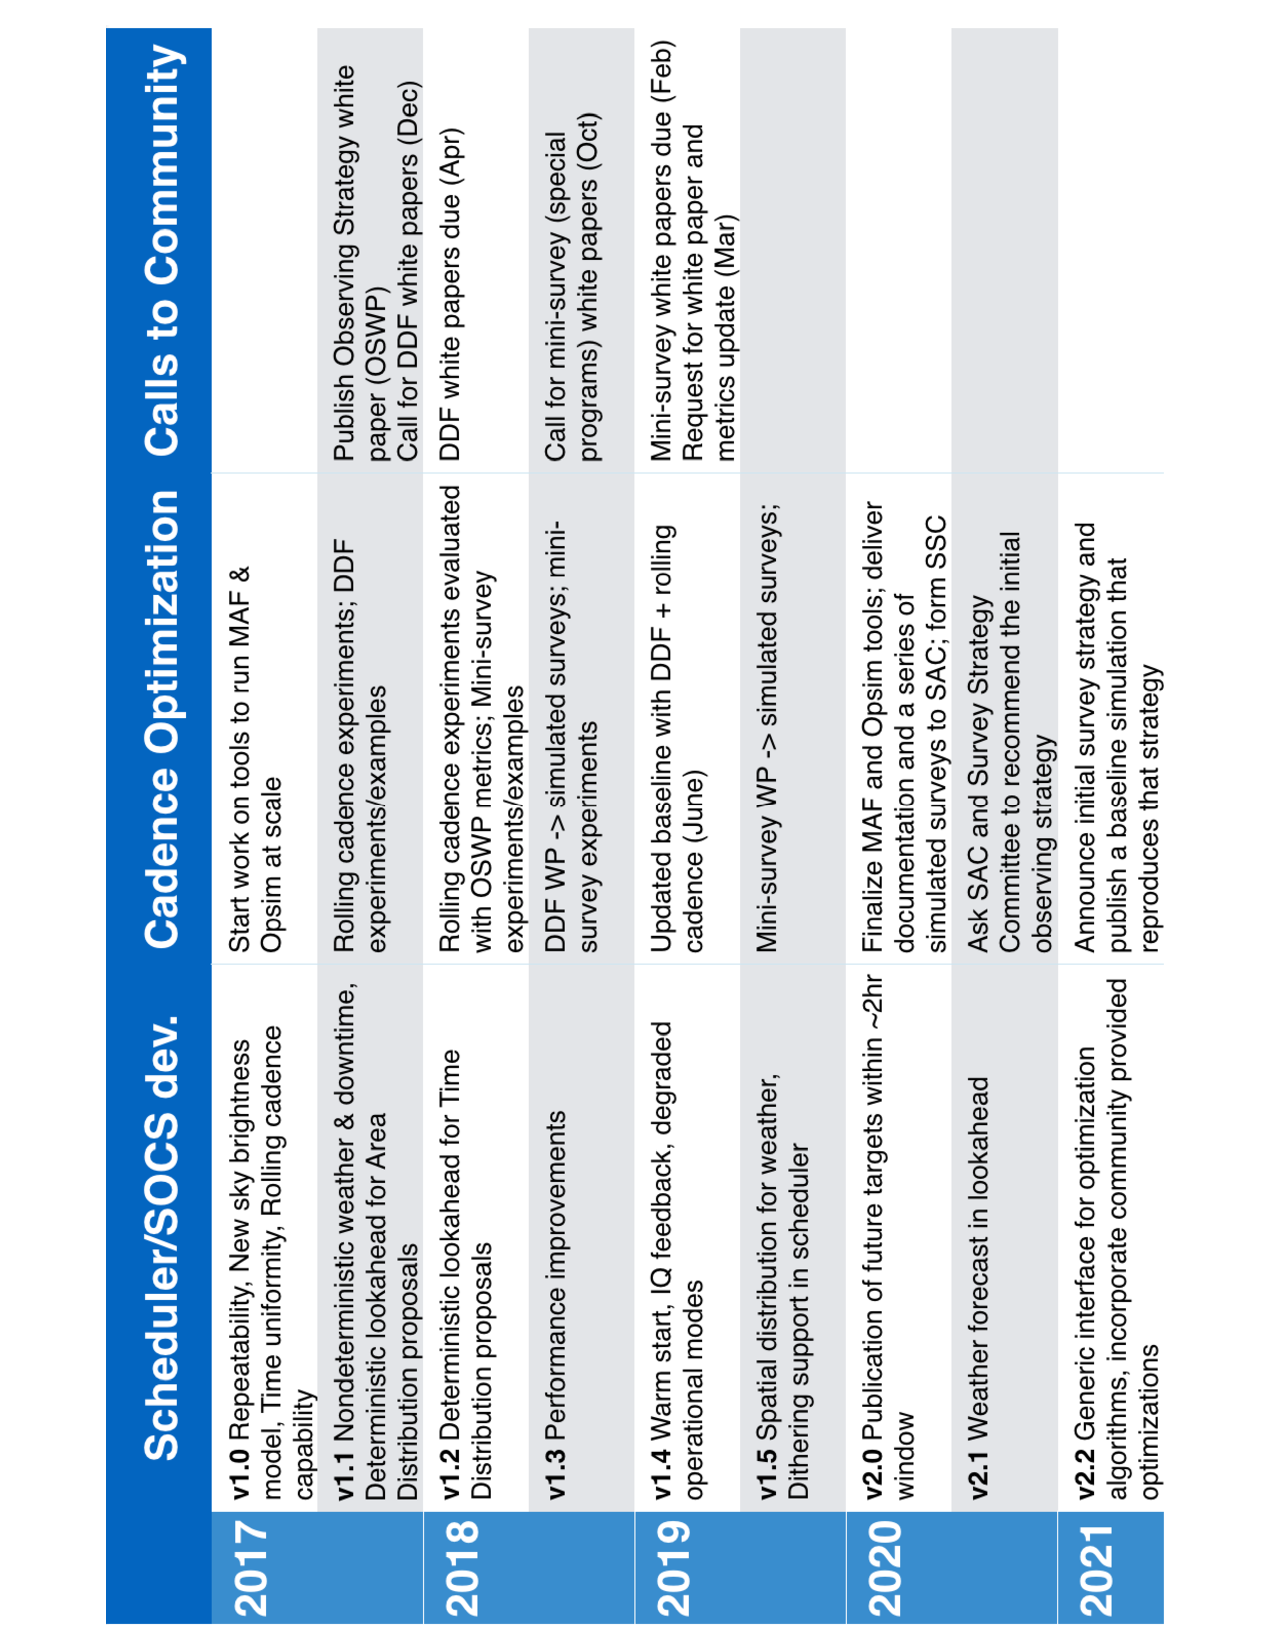
\includegraphics[angle=0,width=0.9\linewidth,clip]{figs/opsim_timeline.pdf}
\caption{Target timeline for the iterated optimization of the LSST observing strategy through 2020.}
\label{fig:timeline}
\end{figure}
%%%%%%%%%%%%%%%%%%%%%%%%%%%%%%%%%

It's important to note that the dates for this timeline are {\it
targets}. Since the deliverables are dependent on the availability of
project resources, these milestones should be considered as those we
could achieve given our best effort. Likewise, given the limited
availability of resources in the SOCS and Scheduler engineering team,
support of community members who wish to use \OpSim v4 will be on a best
effort basis. \OpSim v4 will be delivered as a Docker container and its
use and operation will be documented, but there will be no guarantee of
support for, or timeliness in response to requests for support from,
community users. The solution to this problem is to work together: the LSST Observing Strategy community, represented here by this white paper, is already developing the skills to perform and analyze LSST operations simulations: by learning from each other, we can produce high quality quantitative conclusions for the Project to act upon.



\navigationbar


% --------------------------------------------------------------------

\section{Guidelines for Contributors}
\def\secname{guidelines}\label{sec:\secname}

\credit{drphilmarshall}

Contributions to this community effort are welcome from everyone. In
this section we give brief guidelines for how to make a contribution,
and how you should structure that contribution.

\subsection{How to Get Involved}

The first thing you should do is browse the current version of the white
paper, which you should be able to \href{http://ls.st/iw2}{view on
\GitHub}. You can download the  continuously-compiled
\href{http://www.slac.stanford.edu/~digel/ObservingStrategy/whitepaper/LSST_Observing_Strategy_White_Paper.pdf}{latest
version of the PDF document}, which is hyper-linked for easy navigation.
You will then be able to provide good feedback, which you should do via
the
\href{https://github.com/LSSTScienceCollaborations/ObservingStrategy/issues}{\GitHub
issues}. Please search the existing issues first: there might be a
conversation already taking place that you could join. New issues are
most welcome: we'd like to make this white paper as comprehensive as
possible.

To edit the white paper, you'll need to
\href{https://help.github.com/articles/fork-a-repo/}{``fork'' its
repository}. You will then  be able to edit the paper in your own
fork, and when you are ready,  submit a
\href{https://help.github.com/articles/using-pull-requests/}{``pull
request''} explaining what you are doing and the new version that  you
would like to be accepted. It's a good idea to submit this pull
request sooner rather than later, because associated with it will be a
discussion thread that the writing community can use to discuss your
ideas with you. For help getting started with \git and \GitHub, please
see this
\href{https://github.com/drphilmarshall/GettingStarted#top}{handy
guide}.


\subsection{Writing Science Cases}

For a high-level justification of the following design, please see
\autoref{sec:intro:evaluation} above. In short, we're aiming for modular
science sections (that are easy to write in parallel, and then
re-arrange into other publications later) that are each focused on {\it
one science project each}, and quantified by one (or maybe two) Figures
of Merit (which will likely depend on other, lower-level diagnostic
metrics).

At the beginning of each science chapter there will be a brief
\textit{introduction} that outlines the commonality of the key science
projects contained in that chapter. The individual science sections
following this introduction will then need to describe the particular
discoveries and measurements that are being targeted in each
\textit{science case}.

It will be helpful to think of these science
cases as investigations that the section leads {\it actually plan to
do}. Thinking this way means that each individual section can follow the
tried and tested format of an {\it observing proposal}: a brief
description of the investigation, with references, followed by subsections
describing the analysis
of its technical feasibility. The latter is where the \MAF analysis
should go. Like an observing proposal, each section will seek to
demonstrate the science performance achievable given various assumptions
about the time that could be awarded, or in our case, the survey that
could be delivered.

For an example of how all this could look, please see the
\hyperref[sec:lenstimedelays]{lens time delays section}. While the \MAF
analysis in this science case is still in progress, the suggested
structure of the science case can be seen. Template latex files for the
chapters and sections can be found in the
\href{https://github.com/LSSTScienceCollaborations/ObservingStrategy}{\GitHub
repository}.


\subsection{Metric Quantification}
\label{sec:\secname:metrics}

The feasibility of each science case will need to be quantified using
the \MAF framework, via a set of metrics (a Figure of Merit, and some
diagnostic metrics)  that need to be computed for any given observing
strategy in order to quantify the impact of that cadence on the
described science.

In many (or perhaps all) cases, a Figure of Merit will be a
\textit{precision} (\ie a percentage statistical uncertainty) on a
astrophysical model parameter, assuming negligible bias in its
inference. Precision is usually what we need to forecast in order to
convince TAC's to give us telescope time, and so it makes sense to focus
on it here too.

Early on in a metric analysis, it may not be possible to compute a
science case's Figure of Merit, most likely because to do do would
require a large simulation program to capture the response of the
parameter measurement to the observing strategy. At this early stage, it
makes sense to look for simple {\it proxies} that scale the same way as
model parameter precision. For example, we might expect the precision on
a set of luminosity function  parameters to scale with the square root
of the number of objects in the sample, and so $\sqrt{N}$ could be a
sensible proxy for the Figure of Merit. Provided we get the scaling
right, we can then compare different observing strategies by looking  at
{\it the percentage change in the Figure of Merit,} and arguing that
this will correspond approximately to the same percentage change in the
ideal case.

Each science section needs to conclude with a discussion of any risks
that have been identified, and how these could be mitigated. What does
this mean? Each science project will have a threshold acceptable
Figure of Merit value, as well as a target (or ``design'') value.  If
an observing strategy gives an FoM value below the threshold, it
is very important that we know about it.  Optimizing all science cases
in such a complex and diverse set is not really the best way of
thinking about LSST's scheduling task: rather than maximizing
happiness, what we are really trying to do is minimize global
unhappiness.
The comparisons between different simulated strategies will help make
the case for any changes to the baseline strategy, and in the short term
provide motivation for
\href{https://github.com/LSSTScienceCollaborations/ObservingStrategy/blob/master/opsim/README.md}{proposed
new \OpSim simulation runs.}

For some science sections we will have only a metric design, without an
implementation. As this white paper  evolves, many of these designs will
be realized and put into action. At first, though, the discussion of
risks to these science cases will necessarily be minimal, containing
only predictions for how the Figure of Merit is likely to vary among
observing strategies. These ``ideas'' sections will be presented as
sub-sections of a ``Future Work'' section, on the grounds that the
quantitative analysis is still to come. As its \MAF-based evaluation and
investigation proceeds, a science case will graduate into the main
part of the chapter and become a ``results'' section. The results
sections are clearly visible from the Table of
Contents. To find a Future Work subsection on any particular topic,
you can use the search facility on your PDF viewer.

When does an  ``ideas'' section become a ``results'' section? {\it As
soon as science  performance is quantified using any of the outputs from
\OpSim.} There is  a learning curve associated with the \MAF, but
metrics should be able to be designed before the \MAF documentation is
even opened. And since \MAF metrics always work with \OpSim outputs, any
quantitative analysis that is focused towards those outputs will have
the potential to grow into one of the \MAF analyses we need.


\subsection{Proposing New Simulations}

Before we can optimize the LSST observing strategy we must first
evaluate its current version for all the science cases we care about.
The logical point at which to propose a new \OpSim simulation, capturing
a novel aspect of the observing strategy, is {\it after} evaluating the
baseline  cadence (and others). The discussion section of your science
case is a good place to suggest new \OpSim simulations for further
testing by the community; there is also an
\href{https://github.com/LSSTScienceCollaborations/ObservingStrategy/blob/master/opsim/README.md}{online
suggestion board} for ideas for new  simulations to be registered and
shared.

\navigationbar

% --------------------------------------------------------------------

\section{Outline of This Paper}
\def\secname{intro:outline}\label{sec:\secname}

The rest of this white paper is structured as follows. In
\autoref{chp:cadexp} we describe a number of \OpSim simulated observing
schedules (``cadences'') explored by the LSST Sims team in summer 2015
in preparation for this paper: they include a ``baseline cadence'', and
then some small but interesting perturbations to it. Then, we present
the science cases considered so far, organised into the following
chapters:

\begin{itemize}
    \item \autoref{chp:solarsystem}: \nameref{chp:solarsystem}
    \item \autoref{chp:galaxy}: \nameref{chp:galaxy}
    \item \autoref{chp:variables}: \nameref{chp:variables}
    \item \autoref{chp:transients}: \nameref{chp:transients}
    \item \autoref{chp:MCs}: \nameref{chp:MCs}
    \item \autoref{chp:agn}: \nameref{chp:agn}
    \item \autoref{chp:cosmo}: \nameref{chp:cosmo}
    \item \autoref{chp:specialsurveys}: \nameref{chp:specialsurveys}
    \item \autoref{chp:wfirst}: \nameref{chp:wfirst}
\end{itemize}

Finally, in \autoref{chp:tradeoffs} we bring the results of all the
science metric analyses  together and discuss the tensions between
them, and the trade-offs that we can anticipate having to make.
This final chapter will serve as this work's set of running conclusions.


\navigationbar


% The following chapter shows a template introduction and
% science case section for you to work from. The latter is checked into
% the repository as
% \href{https://github.com/LSSTScienceCollaborations/ObservingStrategy/blob/master/whitepaper/section-template.tex}{\texttt{section-template.tex}}.
% For an example of a section being developed according to the above guidelines,
% please take a look at \autoref{sec:lenstimedelays}.

% % ====================================================================
%
% \setcounter{chapter}{-1}
% \chapter{Template Science Chapter}
% \def\chpname{example}\label{chp:\chpname}
%
% \noindent {\it
% Editor Name(s)
% }
%
% % --------------------------------------------------------------------
%
% \section{Introduction}
% \label{sec:\chpname:intro}
%
% General introduction to the chapter's science projects.
%
% Overview of observing strategy needed by those projects, bringing
% out common themes or points of tension.
%
% % --------------------------------------------------------------------
%
% \input{section-template}
%
% % --------------------------------------------------------------------
